\documentclass[12pt]{article}
\usepackage{graphicx}
\usepackage[letterpaper,margin=1in]{geometry}
\begin{document}
This document contains a letter that has been folded up inside a bible
that once belonged to Robert Carley, who was born in Ireland and died
in Seguin, Texas, where he was Rector of St.\ Andrews Episcopal
Church.

The letter is addressed to ``Alice,'' who was probably his daughter,
Margaret Alice Carley. If I am deciphering the handwriting correctly,
Robert is writing to Alice on her birthday. About half way down the
first page, he writes ``you will want to be very good now as you have
grown so old---now eight years---what a great girl.'' If only I knew
when Alice was born, this would date the letter. Robert died in 1872
at the age of 38.

Margaret Alice married Robert Glass. My grandmother, Mary Glass
Chamberlain, was one of their many children.

Here is my best effort at a transcription:
\begin{quotation}
  \noindent My dearest Alice,

  I have just [thought?] that this is your birth day, so as I cannot
  be with you to congratulate, I must do what is next best, that is,
  write you a line. You will want to be very good now as you have
  grown so old---now eight years---what a great girl. You will be able
  now to get such perfect lessons, while [or which?] your
  [indecipherable] so big, that your teacher will be very glad
  indeed. And [we?] will all be very glad to [missing] you get on
  nicely, and then [indecipherable] you will go into the common
  school, and that will be something [grand?].

  What fine sunny weather we have. I often wish that I could ask you
  and [Frankie?] [out here?] to enjoy the pleasant sunshine.

  I send you best love and many birth day Kisses.

  Do not forget to be [missing word]. I hope you get along nicely with
  the [indecipherable] and help all you can. [It?] pleases everyone to
  see a little girl [industrious?].

  Give my love to the baby, and give him a Kiss for me.

  It is beautiful to hear the birds sing out here in the woods.

  Your loving father

  \mbox{}\hfill Robert Carley.
\end{quotation}
I would welcome corrections or additions to this transcription


\bigskip

\mbox{}\hfill Alan R. Rogers\\
\mbox{}\hfill sregorra@gmail.com\\

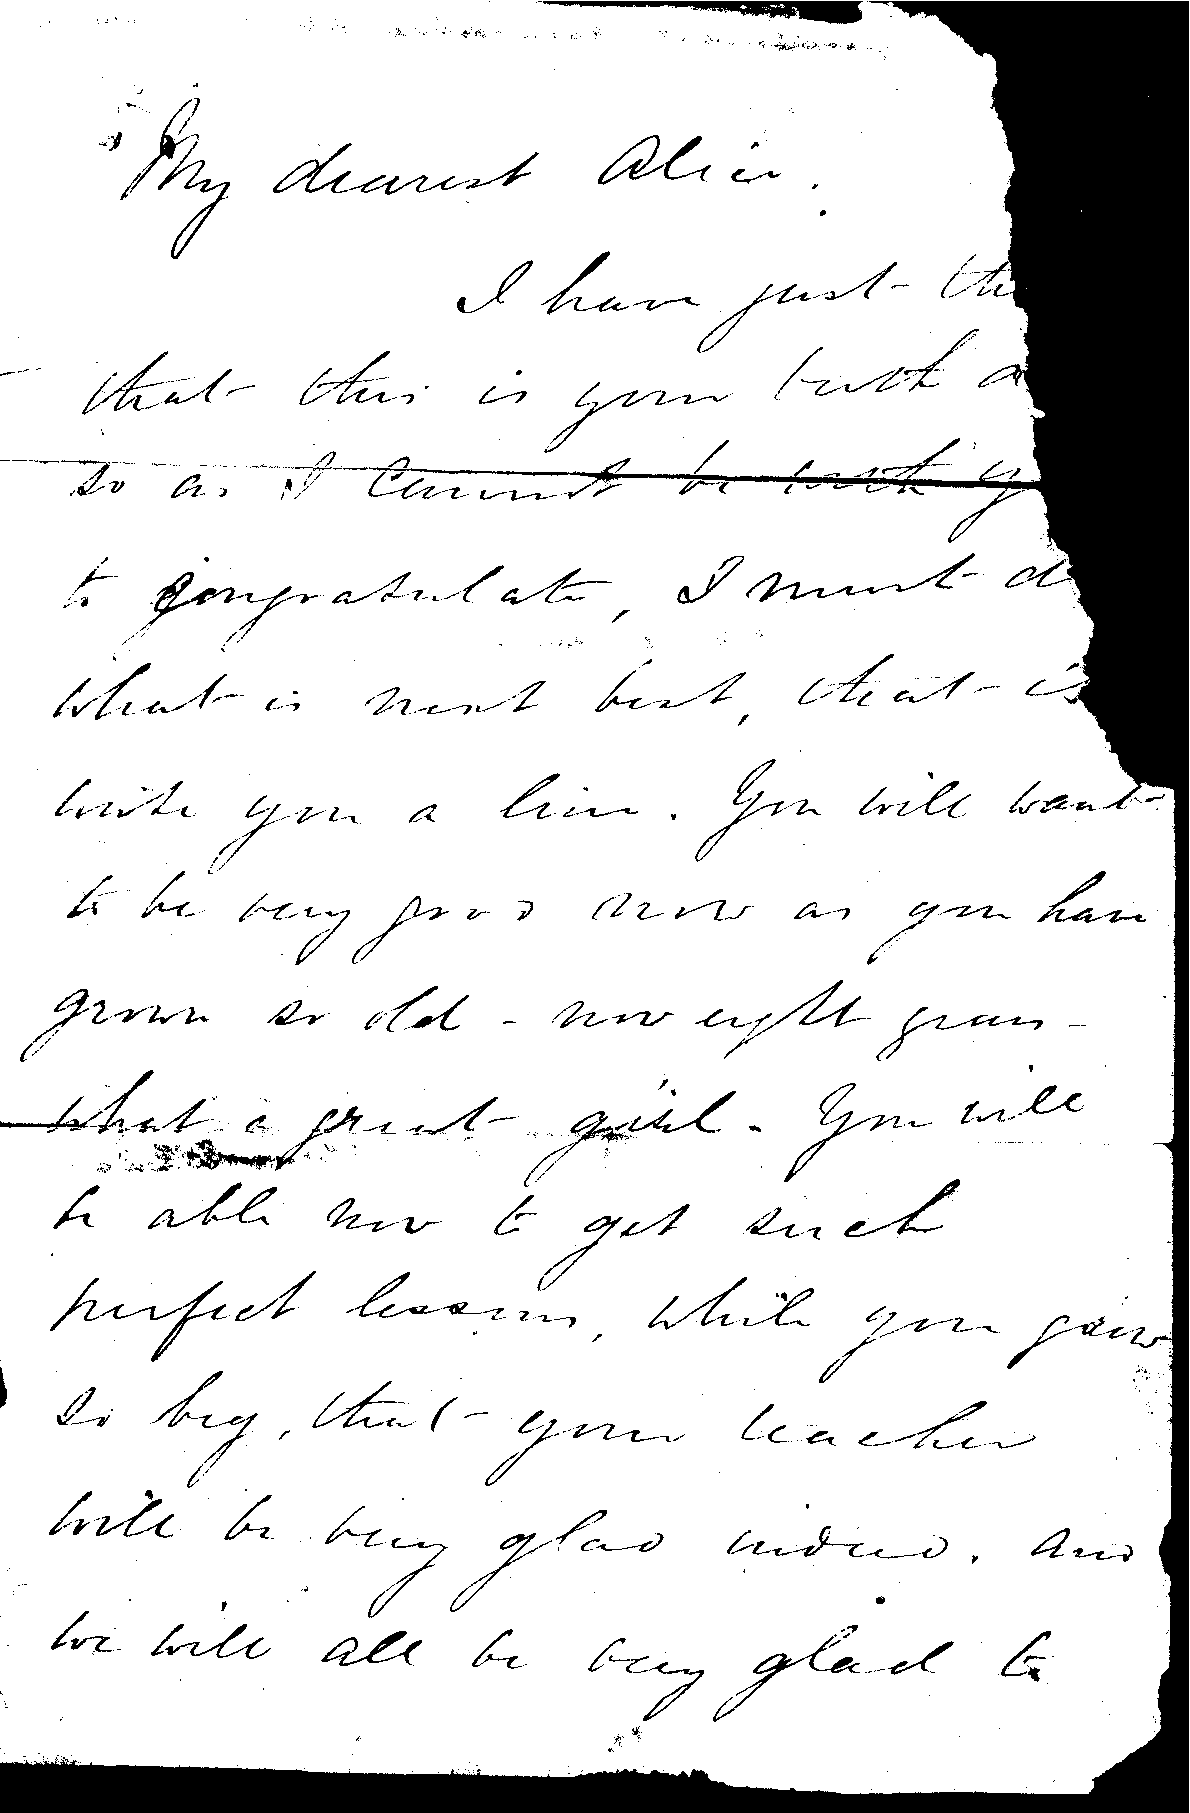
\includegraphics[width=\textwidth]{RobtCarley1.pdf}
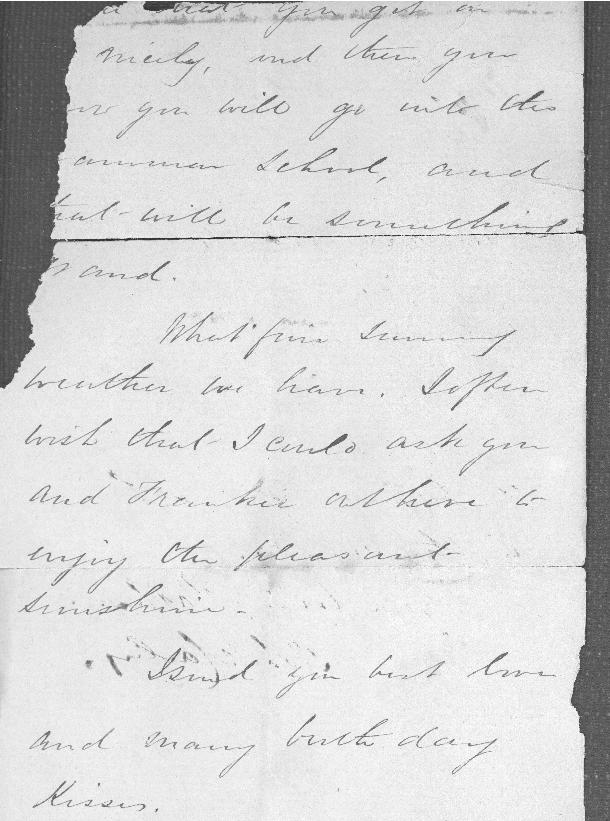
\includegraphics[width=\textwidth]{RobtCarley2.pdf}
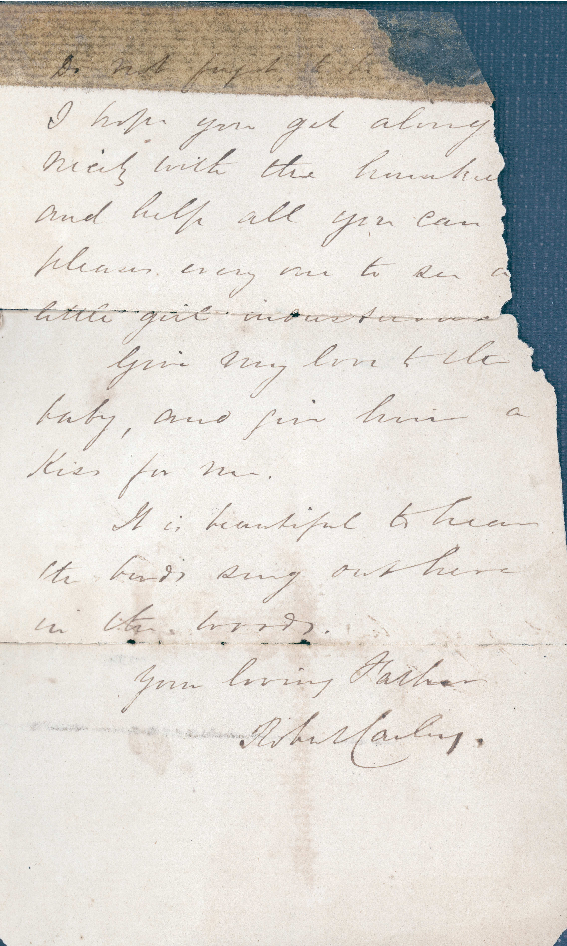
\includegraphics[width=\textwidth]{RobtCarley3.pdf}
\end{document}
